\documentclass[thesis=B,czech]{FITthesis}[2012/06/26]

\usepackage[utf8]{inputenc}
\usepackage{graphicx}
\usepackage{dirtree}
\usepackage{float}
\usepackage{color}
\usepackage{listings}

\lstdefinelanguage{RainerScript}
{
  morekeywords={
    module, if, then, while, for, load, set, unset,
	template, name, type, string, action, stop, and,
    from, to, var, stringtobedeleted, severity
  },
  sensitive=false,
  morecomment=[l]{\#},
  morecomment=[s]{/*}{*/},
  morestring=[b]"
}

\lstdefinelanguage{PKGBuild}
{
  morekeywords={
    pkgname, pkgver, arch, depends, source, md5sums,
    build, package
  },
  sensitive=false,
  morecomment=[l]{\#},
  morecomment=[s]{/*}{*/},
  morestring=[b]"
}

%\lstdefinestyle{numbers} {numbers=left, stepnumber=1, numberstyle=\tiny, numbersep=10pt}
%\lstdefinestyle{MyFrame}{backgroundcolor=\color{white},frame=shadowbox}



\lstdefinestyle{AshStyle} %{language=Bash,style=numbers,style=MyFrame,frame=none,backgroundcolor={}}
{language=Bash,                % choose the language of the code
basicstyle=\footnotesize,       % the size of the fonts that are used for the code
numbers=left,                   % where to put the line-numbers
numberstyle=\footnotesize,      % the size of the fonts that are used for the line-numbers
stepnumber=1,                   % the step between two line-numbers. If it is 1 each line will be numbered
numbersep=5pt,                  % how far the line-numbers are from the code
backgroundcolor=\color{white},  % choose the background color. You must add \usepackage{color}
showspaces=false,               % show spaces adding particular underscores
showstringspaces=false,         % underline spaces within strings
showtabs=false,                 % show tabs within strings adding particular underscores
frame=single,           % adds a frame around the code
tabsize=2,          % sets default tabsize to 2 spaces
captionpos=b,           % sets the caption-position to bottom
breaklines=true,        % sets automatic line breaking
breakatwhitespace=false,    % sets if automatic breaks should only happen at whitespace
escapeinside={\%*}{*)}          % if you want to add a comment within your code
}

\lstdefinestyle{RainerScriptSimpleStyle} %{language=Bash,style=numbers,style=MyFrame,frame=none,backgroundcolor={}}
{language=RainerScript,                % choose the language of the code
basicstyle=\footnotesize,       % the size of the fonts that are used for the code
backgroundcolor=\color{white},  % choose the background color. You must add \usepackage{color}
showspaces=false,               % show spaces adding particular underscores
showstringspaces=false,         % underline spaces within strings
showtabs=false,                 % show tabs within strings adding particular underscores
frame=lines,           % adds a frame around the code
tabsize=2,          % sets default tabsize to 2 spaces
captionpos=b,           % sets the caption-position to bottom
breaklines=true,        % sets automatic line breaking
breakatwhitespace=false,    % sets if automatic breaks should only happen at whitespace
escapeinside={\%*}{*)}          % if you want to add a comment within your code
}

\lstdefinestyle{RainerScriptStyle} %{language=Bash,style=numbers,style=MyFrame,frame=none,backgroundcolor={}}
{language=RainerScript,                % choose the language of the code
basicstyle=\footnotesize,       % the size of the fonts that are used for the code
numbers=left,                   % where to put the line-numbers
numberstyle=\footnotesize,      % the size of the fonts that are used for the line-numbers
stepnumber=1,                   % the step between two line-numbers. If it is 1 each line will be numbered
numbersep=5pt,                  % how far the line-numbers are from the code
backgroundcolor=\color{white},  % choose the background color. You must add \usepackage{color}
showspaces=false,               % show spaces adding particular underscores
showstringspaces=false,         % underline spaces within strings
showtabs=false,                 % show tabs within strings adding particular underscores
frame=single,           % adds a frame around the code
tabsize=2,          % sets default tabsize to 2 spaces
captionpos=b,           % sets the caption-position to bottom
breaklines=true,        % sets automatic line breaking
breakatwhitespace=false,    % sets if automatic breaks should only happen at whitespace
escapeinside={\%*}{*)}          % if you want to add a comment within your code
}

\lstdefinestyle{PKGBuildStyle} %{language=Bash,style=numbers,style=MyFrame,frame=none,backgroundcolor={}}
{language=PKGBuild,                % choose the language of the code
basicstyle=\footnotesize,       % the size of the fonts that are used for the code
numbers=left,                   % where to put the line-numbers
numberstyle=\footnotesize,      % the size of the fonts that are used for the line-numbers
stepnumber=1,                   % the step between two line-numbers. If it is 1 each line will be numbered
numbersep=5pt,                  % how far the line-numbers are from the code
backgroundcolor=\color{white},  % choose the background color. You must add \usepackage{color}
showspaces=false,               % show spaces adding particular underscores
showstringspaces=false,         % underline spaces within strings
showtabs=false,                 % show tabs within strings adding particular underscores
frame=single,           % adds a frame around the code
tabsize=2,          % sets default tabsize to 2 spaces
captionpos=b,           % sets the caption-position to bottom
breaklines=true,        % sets automatic line breaking
breakatwhitespace=false,    % sets if automatic breaks should only happen at whitespace
escapeinside={\%*}{*)}          % if you want to add a comment within your code
}


\department{Katedra softwarového inženýrství}
\title{Flexibilní logování pro embedded Linuxové systémy}
\authorGN{David}
\authorFN{Vavřička}
\authorWithDegrees{David Vavřička}
\supervisor{Ing. Matěj Laitl}
\acknowledgements{Doplňte, máte-li komu a za co děkovat. V~opačném případě úplně odstraňte tento příkaz.}
\abstractCS{Doplňte}
\abstractEN{Sem doplňte ekvivalent abstraktu Vaší práce v~angličtině.}
\placeForDeclarationOfAuthenticity{V~Praze}
\declarationOfAuthenticityOption{4} %volba Prohlášení (číslo 1-6)
\keywordsCS{logování, vestavěné systémy, logovací démoni, Linux, Rsyslog}
\keywordsEN{logging, embedded systems, logging daemons, Linux, Rsyslog}

\begin{document}

\begin{introduction}

\end{introduction}

\chapter{Technické požadavky}
Cílem je upravit logovací řešení pro set-top box EKT DID7006mTF~\cite{ekt7006} tak, aby splňovalo technické požadavky popsané v této kapitole. Řešení musí fungovat a být otestováno na zmíněném modelu set-top boxu a pokud možno by mělo být přenositelné i na jiné typy set-top boxů.
Požadavky jsou rozděleny na základní a rozšířené. Rozšířené požadavky není nutno implementovat.

\section{Základní technické požadavky}

\subsection{Snížení objemu logů}
Je žádoucí umožnit snížit objem zasílaných logů z důvodu přílišného zatížení sítě a serverových disků. A to tak, že zadavatel bude schopen nadefinovat pro každou komponentu úroveň severity zpráv, od které mají být posílány na server. Výchozí nastavení dodá zadavetel.

\subsection{Vzdálená konfigurace}
Technické řešení musí být schopno za běhu pomocí SHELL-ového API měnit maximální severitu zpráv pro jednotlivé komponenty a dále toto API musí umožnit nastavit výchozí severitu, která se použije pro komponenty ji nemají explicitně nastavenou. Takto změněné nastavení musí být perzistentní i po restartu STB. Výchozí nastavení se obnoví až po factory resetu. API navrhne dle své libovůle sám řešitel.

\subsection{Rate-limiting odesílaných zpráv}
Nové logovací řešení musí být schopné provádět rate-limiting odesílanych zpráv tak, aby nepřekročilo maximální vyhrazenou šířku pásma. Naivní rate-limiting je i v existujícím řešení, řešitel navrhne výchozí nastavení nového řešení tak, aby přibližně odpovídalo současnému chování. 

\subsection{Formát logů}
Je nutno zachovat formát logů jako ho má původní řešení, aby se jednalo o drop-in replacement bez nutnosti jakkoli měnit konfiguraci serveru, který sbírá logy od set-top boxů.

\subsection{Razítkování zpráv}
Každé zprávě se musí přidat textový prefix id=N, kde N monotonicky roste s každou zprávou.  To slouží pro detekci ztracených zpráv. Id přeteče po dvaceti bitech. Po rebootu STB id znovu začíná od 1.

\subsection{Post-processing zpráv}
Zadavatel má pouze částečnou kontrolu nad zprávami generovanými aplikacemi na set-top boxu, například nedokáže ve všech případech eliminovat dlouhé prefixy u zpráv. Je proto nutno takové prefixy rozpoznat a vhodně odfiltrovat před odesláním. Ze stejného důvodu mají některé zprávy nevhodně vyplněnou severitu a položku app-name. Jejich správné hodnoty jsou uloženy v textu zprávy, jejíž formát je pro jednotlivé skupiny zpráv konstantní. Řešení bude schopné tyto údaje z těla zprávy extrahovat a nahradit jimi původní metadata. Tato pravidlo musí být možné definovat a měnit bez nutnosti nového sestavení softwaru. 
Řešitel vytvoří pro ukázku 3 pravidla, která budou sloužit zadavateli jako šablony pro možná budoucí filtrovací pravidla.

\section{Rozšířené technické požadavky}

\subsection{Komprese zpráv}
Bylo by vhodné zvážit pro a proti komprese zpráv. Vyplatí se ušetřená přenesená data oproti režiji spojené s kompresí a dekompresí zpráv?

\chapter{Logování v linuxových systémech}
Systémoví administrátoři se musí umět vypořádat s množstvím nejrůznějších zpráv ze systémových komponent nebo například ze vzdálených systémů.
Pro jejich snažší správu slouží na UNIX-ových a tedy i LINUX-ových systémech tzv. Syslog.
Tím je myšlen Syslog formát zpráv, který zprávám dává unifikovanou podobu.
Dále je tím myšlen Syslog protokol, tedy specifikace pro přenos Syslog zpráv po síti.

\section{Syslog démon}
Démon je v UNIXovém světě označení pro takový proces, který oproti běžným procesům neintereaguje přímo s uživatelem, ale běží na pozadí operačního systému a funguje samostatně. Hlavním účelem syslog démona je sběr logů od ostatních procesů, které následně v závislosti na jeho konfiguraci dokáže filtrovat a ukládat na disk či odesílat na vzdálený server.

\section{Syslog protokol}
Syslog protokol~\cite{NetworkAdmSurGuide} spatřil světlo světa již v roce 1980. Má ho na svědomí Eric Allman, který jej psal s úmyslem využít ho pro potřeby Sendmail projektu. Nicméně postupem času byl tento protokol díky skvělému návrhu a díky své jednoduchosti adaptován i jinými projekty. Rozšířil se na různé OS a později se stal standardem pro logování na většině Unixových systémů.
Tento protokol poskytuje možnost zařízením posílat notifikační zprávy ať už skrze sít a nebo lokálně v rámci jednoho zařízení na syslog server, kterým je již v minulé kapitole zmíňený syslog démon.

\subsection{The BSD syslog Protocol - RFC 3164}
Až po přibližně 20-ti letech od vzniku syslog protokolu sepsal Chris Lonvick dokument RFC3146~\cite{RFC3164} popisující daný protokol. Do té doby existovala velká spousta v detailech se lišících implementací, což mělo za následek v jistých případech nekompatibilitu. Dokument čítá celkem 19 stránek kde je především detailně popsán formát a parametry zpráv.

\subsection{The Syslog Protocol - RFC 5424}
Oficiální standard vznikl až s příchodem Syslog protokolu RFC 5424, který světu představil v roce 2009 jeho autor Rainer Gerhards. Počet stránek se rozrostl na 37 a došlo k některým zásadním a velice užitečným změnám.

Nový standard umožňuje použití libovolného trasnportního protokolu~\cite{RFC5424-TrProt}, oproti RFC 3164, kde je jako transportní protokol pevně určeno UDP~\cite{RFC3164-UDP}.
Mírných změn doznal také formát zpráv, který je možno strukturovaně rozšiřovat dle specifických potřeb~\cite{RFC5424-MsgForm}. To má ovšem za následek jeho zpětnou nekompatibilitu s RFC~3164.

\section{Syslog formát zpráv}
\begin{figure}[H]
	\centering
	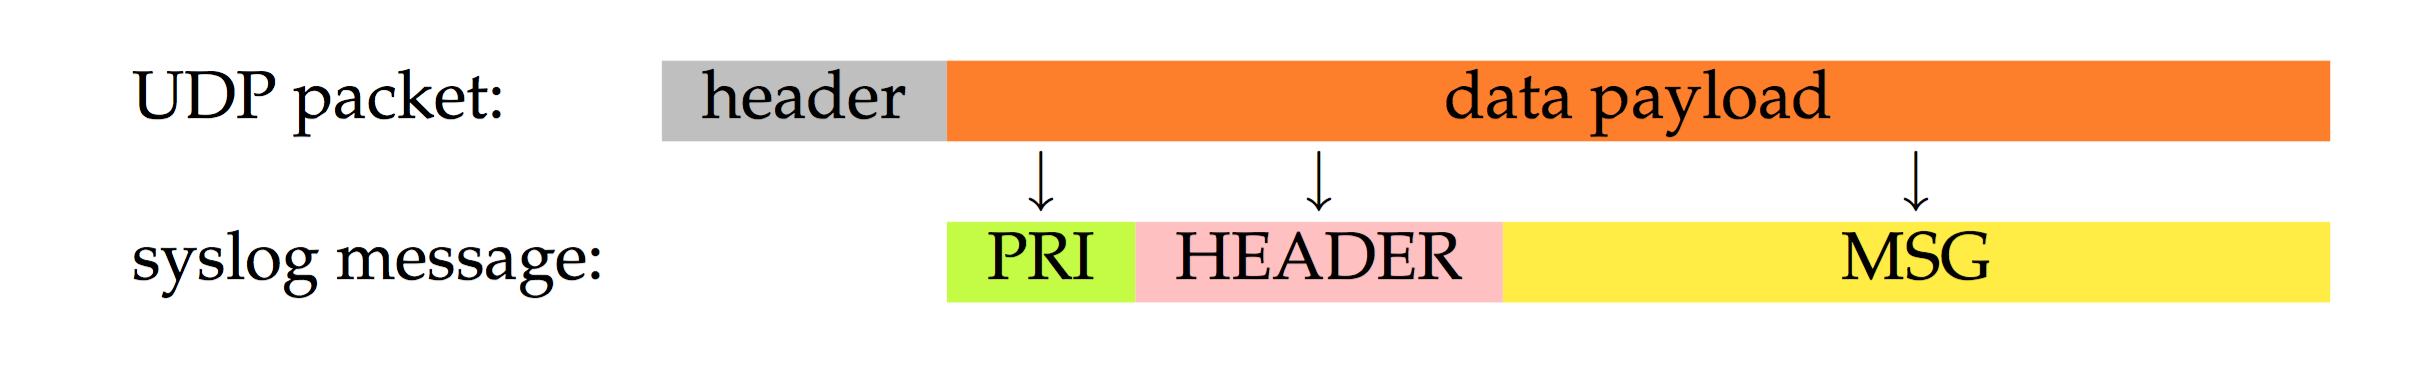
\includegraphics[scale=0.3]{images/syslog-message-format}
	\caption[Formát syslog zprávy]{Formát syslog zprávy}
\end{figure}

Syslog zpráva se skládá ze 3 částí jak je pro lepší představu graficky vyobrazeno na obrázku výše.

\subsection{Část PRI}
PRI se skládá z jedno až tří-místného decimálního čísla PRIVAL ohraničeného symboly~\uv{<}~na začátku a~\uv{>}~na konci.
PRIVAL má v sobě zakódované číselné hodnoty parametrů zprávy označovaných jako Severity a Facility.


$$Prival= 8*Facility+Severity$$


Facility určuje zdroj logů a Severity jejich důležitost (tedy zda se jedná například pouze o debug hlášku nebo naopak o důležitou zprávu například o pádu programu). Na základě těchto dvou hodnot syslog démon provádí základní filtraci zpráv.
Důležitým poznatkem je, že formát PRI je shodný podle dokumentů RFC 5424 i 3164.

\begin{table}[ht]
\centering
	\caption[Tabulka severit podle RFC 3164]{Seznam severit dle RFC 3164.~\cite{RFC3164}}
	\begin{tabular}{|l|l|l|}\hline
		Číselný kód	& Severity & Význam	\tabularnewline \hline \hline
		0		& Emergency	&	Systém je nepoužitelný \tabularnewline \hline
		1		& Alert		&	Vyžadována okamžitá reakce \tabularnewline \hline
		2		& Critical	&	Kritický stav \tabularnewline \hline
		3		& Error		&	Chybový stav	\tabularnewline \hline
		4		& Warning	&	Upozornění na hrozící chybu \tabularnewline \hline
		5		& Notice		&	Neobvyklý stav, ale ne chybový \tabularnewline \hline
		6		& Informational & Informační zpráva \tabularnewline \hline
		7		& Debug		&	Debugovací zpráva \tabularnewline \hline
	\end{tabular}
\end{table}

\begin{table}[ht]   %[H] místo [ht] aby to bylo přesně na daném místě
\centering
	\caption[Tabulka facilit podle RFC 3164]{Seznam facilit dle RFC 3164.~\cite{RFC3164}}
	\begin{tabular}{|l|l|l|}\hline
		Číselný kód & Facility & Původ zpráv \tabularnewline \hline \hline
		0		& kern & Zprávy jádra systému	\tabularnewline \hline
		1		& user & Generované uživatelem	\tabularnewline \hline
		2		& mail & Generované emailovým systémem			\tabularnewline \hline
		3		& daemon & Systémoví démoni			\tabularnewline \hline
		4		& auth & Zprávy autorizačního/zabezpečovacího charakteru		\tabularnewline \hline
		5		& syslog & Generované syslogem	\tabularnewline \hline
		6		& lpr & Tiskový systém		\tabularnewline \hline
		7		& news & Network news systém		\tabularnewline \hline
		8		& uucp & UUCP systém			\tabularnewline \hline
		9		& cron & Zprávy plánovacího systému Cron			\tabularnewline \hline
		10		& security & security/authorization messages			\tabularnewline \hline
		11		& ftp & FTP démon				\tabularnewline \hline
		12		& ntp & NTP systém			\tabularnewline \hline
		13		& logaudit & Log audit				\tabularnewline \hline
		14		& logalert & Log alert				\tabularnewline \hline
		15		& clock & Clock démon			\tabularnewline \hline
		16		& local0 & Lokální zprávy (0)			\tabularnewline \hline
		17		& local1 & Lokální zprávy (1)			\tabularnewline \hline
		\ldots	& \ldots				\tabularnewline \hline
		23		& local7 & Lokální zprávy (7)			\tabularnewline \hline
	\end{tabular}
\end{table}

\subsection{Header}
Tato část zprávy obsahuje časovou značku a identifikaci zdroje (podle IP adresy nebo hostname). Přesnou podobu Headeru specifikují dokumenty RFC 3164 a 5424 odlišně. Zatímco starší dokument definuje přesnou podobu časové značky, tak novější specifikace dovoluje různé formáty. Díky tomu není zaručena plná zpětná kompatibilita.

\subsection{MSG}
Část Msg pokrývá zbývající část syslog paketu. Obecně tam nalézáme různé zbývající informace o procesu generujícího danou zprávu a pak samozřejmě samotný text zprávy.

\chapter{Analýza a návrh}
\begin{figure}[H]
	\centering
	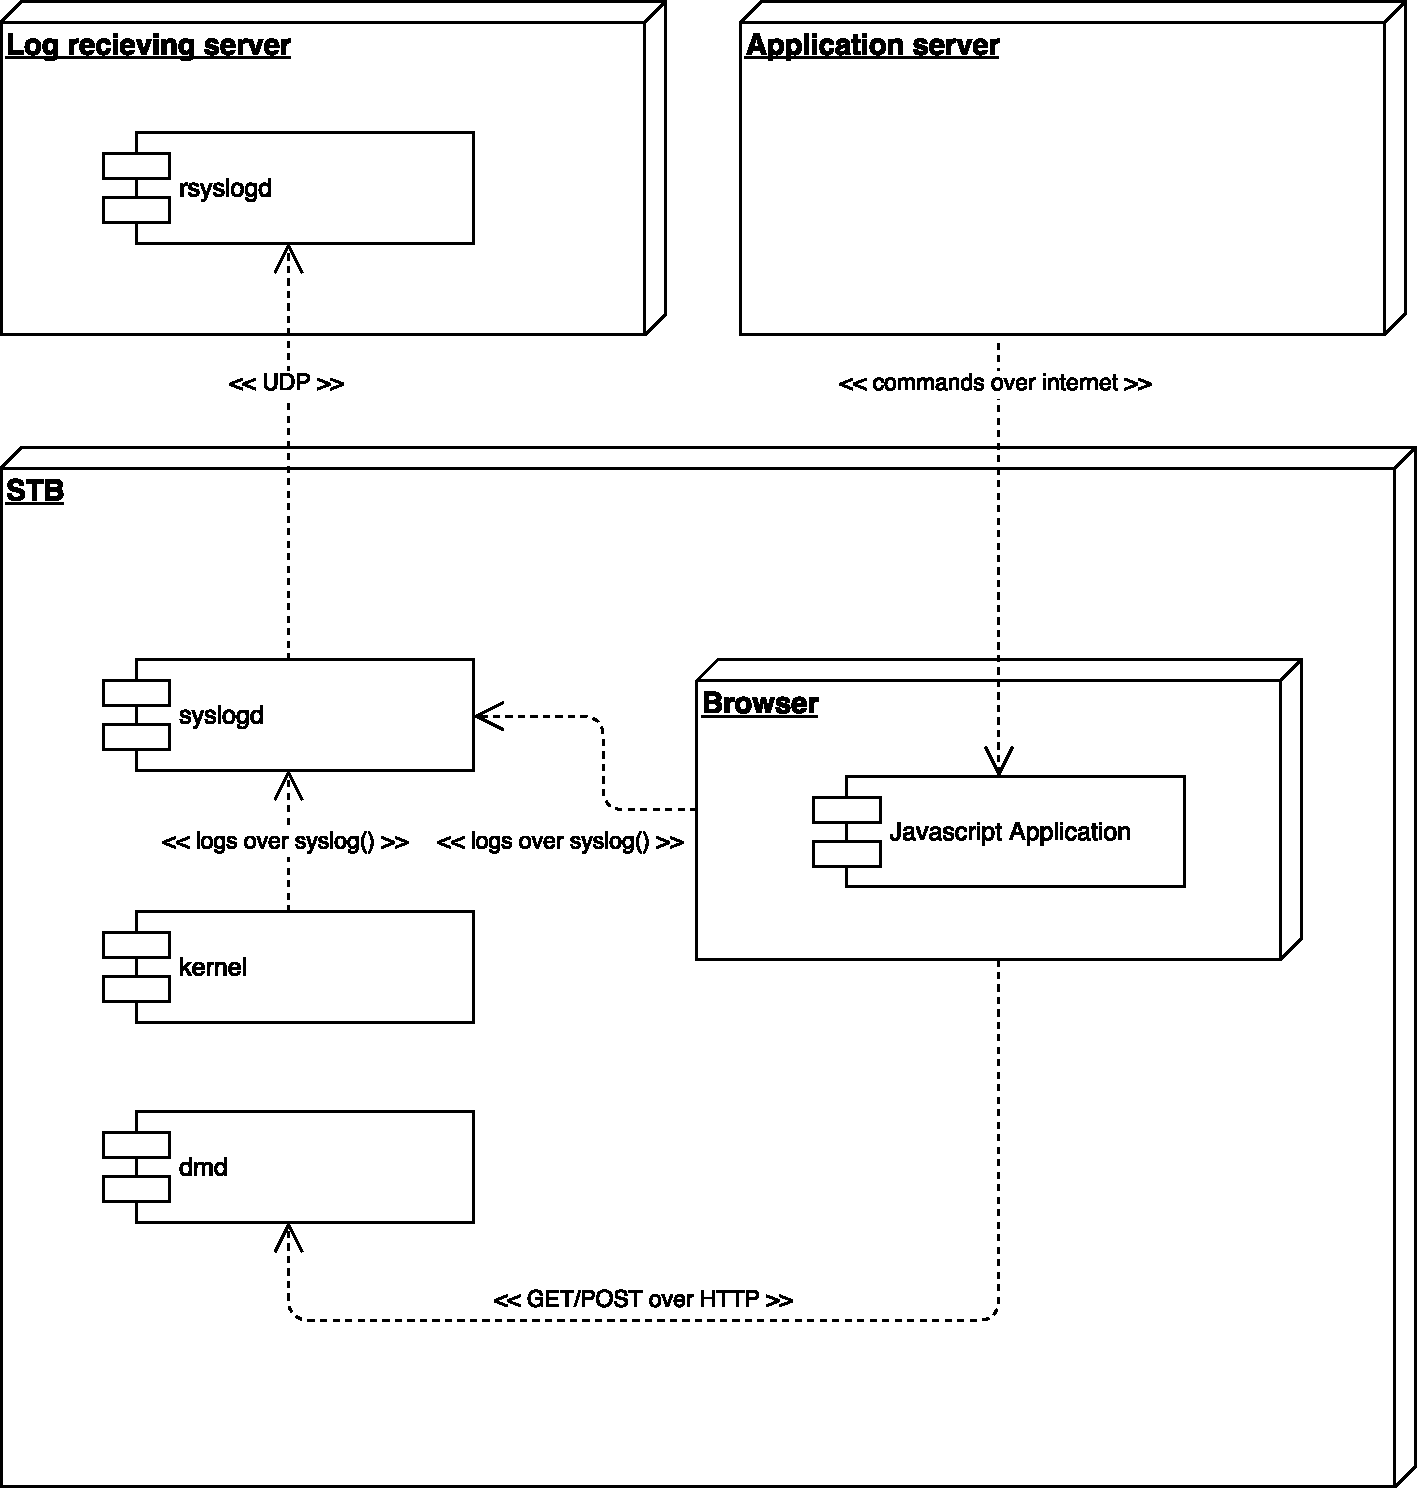
\includegraphics[scale=0.5]{images/diagram-nasazeni-puvodniho-reseni}
	\caption[Diagram nasazení původního řešení]{Diagram nasazení původního řešení}
\end{figure}

\section{Původní řešení}
V této kapitole jsou uvedeny a popsány jednotlivé pro tuto práci důlužité komponenty původního řešení.

\subsection{HW specifikace STB EKT DID7006}
\begin{description}
\setlength\itemsep{-1ex}
  \item [CPU:] ARM 9 Ali M3733 (1GHz Dual core)
  \item [GPU:] Mali 400
  \item [RAM:] 512MB DDR3
  \item [Perzistentní paměť:] 512MB NAND Flash
\end{description}

\subsection{Runtime prostředí}
Na STB běží OS GNU/Linux s Busybox sadou aplikací, která nahrazuje standardní GNU shellové utility. Busybox aplikace jsou díky své malé velikosti vhodnější pro embedded zařízení. Na druhou stranu neobsahují všechny funkcionality a možnosti nastavení.

\subsubsection{Browser}
Browser je jednoduchý internetový prohlížeč dodaný výrobcem STB.
V něm běží v Javascriptu zadavatelem napsaná aplikace poskytující uživatelské rozhraní. Mimo to také naslouchá zprávám z aplikačního serveru, na jejichž základě může provádět akce, a to včetně generování POST či GET requestu pro démon dmd.
Tato javascriptová aplikace spolu s dalším podpogramem nesoucím název player generují velké množství logů. Tyto logy nepoužívají standardizovanou syslog množinu severit, ale svou vlastní s ní nekompatibilní. Logovací démon ovšem očekává zprávy právě podle syslog standardu. Implementaci browseru ani playeru nemůže zadavatel měnit a proto je třeba nekompatibilitu vyřešit pomocí logovacího démonu.

\subsubsection{Servisní komponenta dmd}
Dmd je v C++ napsaná servisní komponenta, která zprostředkovává komunikaci mezi Browserem a shellovým prostředím pomocí minimalistického HTTP serveru. Umožňuje JavaScript aplikaci na STB provádět operace, které jsou dostupné jen z shellového API.

\subsubsection{BusyBox Syslogd}
Jedná se o minimalistický logovací démon, který je podrobněji popsán v následující kapitole \uv{Srovnání logovacích démonů}.
Zadavatel mu pro své potřeby navíc doimplementoval číslování jednotlivých zpráv pro rozpoznání výpadku a za druhé naivní rate-limiting zpráv. Ten je naivní z důvodu, že používá statický buffer na počet zpráv, který nebere ohled na jejich velikost a hlavně bufferované zprávy se neodešlou samy, ale jen s nově příchozími zprávami.
Za použití tohoto démonu není možné splnit některé stěžejní technické požadavky, jako například \uv{Snížení objemu logů} nebo \uv{Post processing zpráv}. Proto bude nutné ho nahradit nějakým vyspělejším démonem. Tím se ale zabývá až další kapitola \uv{Nové řešení}.

\subsection{Aplikační server}
Aplikační server se stará o business logiku, například poskytuje uživateli práva přehrát daný kanál nebo film, komunikuje s javascriptovou aplikací, která se vůči němu autorizuje a podobně.
AS není možné v této práci jakkoli měnit. Je nutné zachovat kompatibilitu.

\subsection{Servery pro sběr logů}
Zadavatel provozuje cluster serverů sbírajících logy od statisíců STB. Běží na nich rsyslog nakonfigurovaný pro co nejlepší výkonost.

\section{Nové řešení}

\begin{figure}[ht]
	\centering
	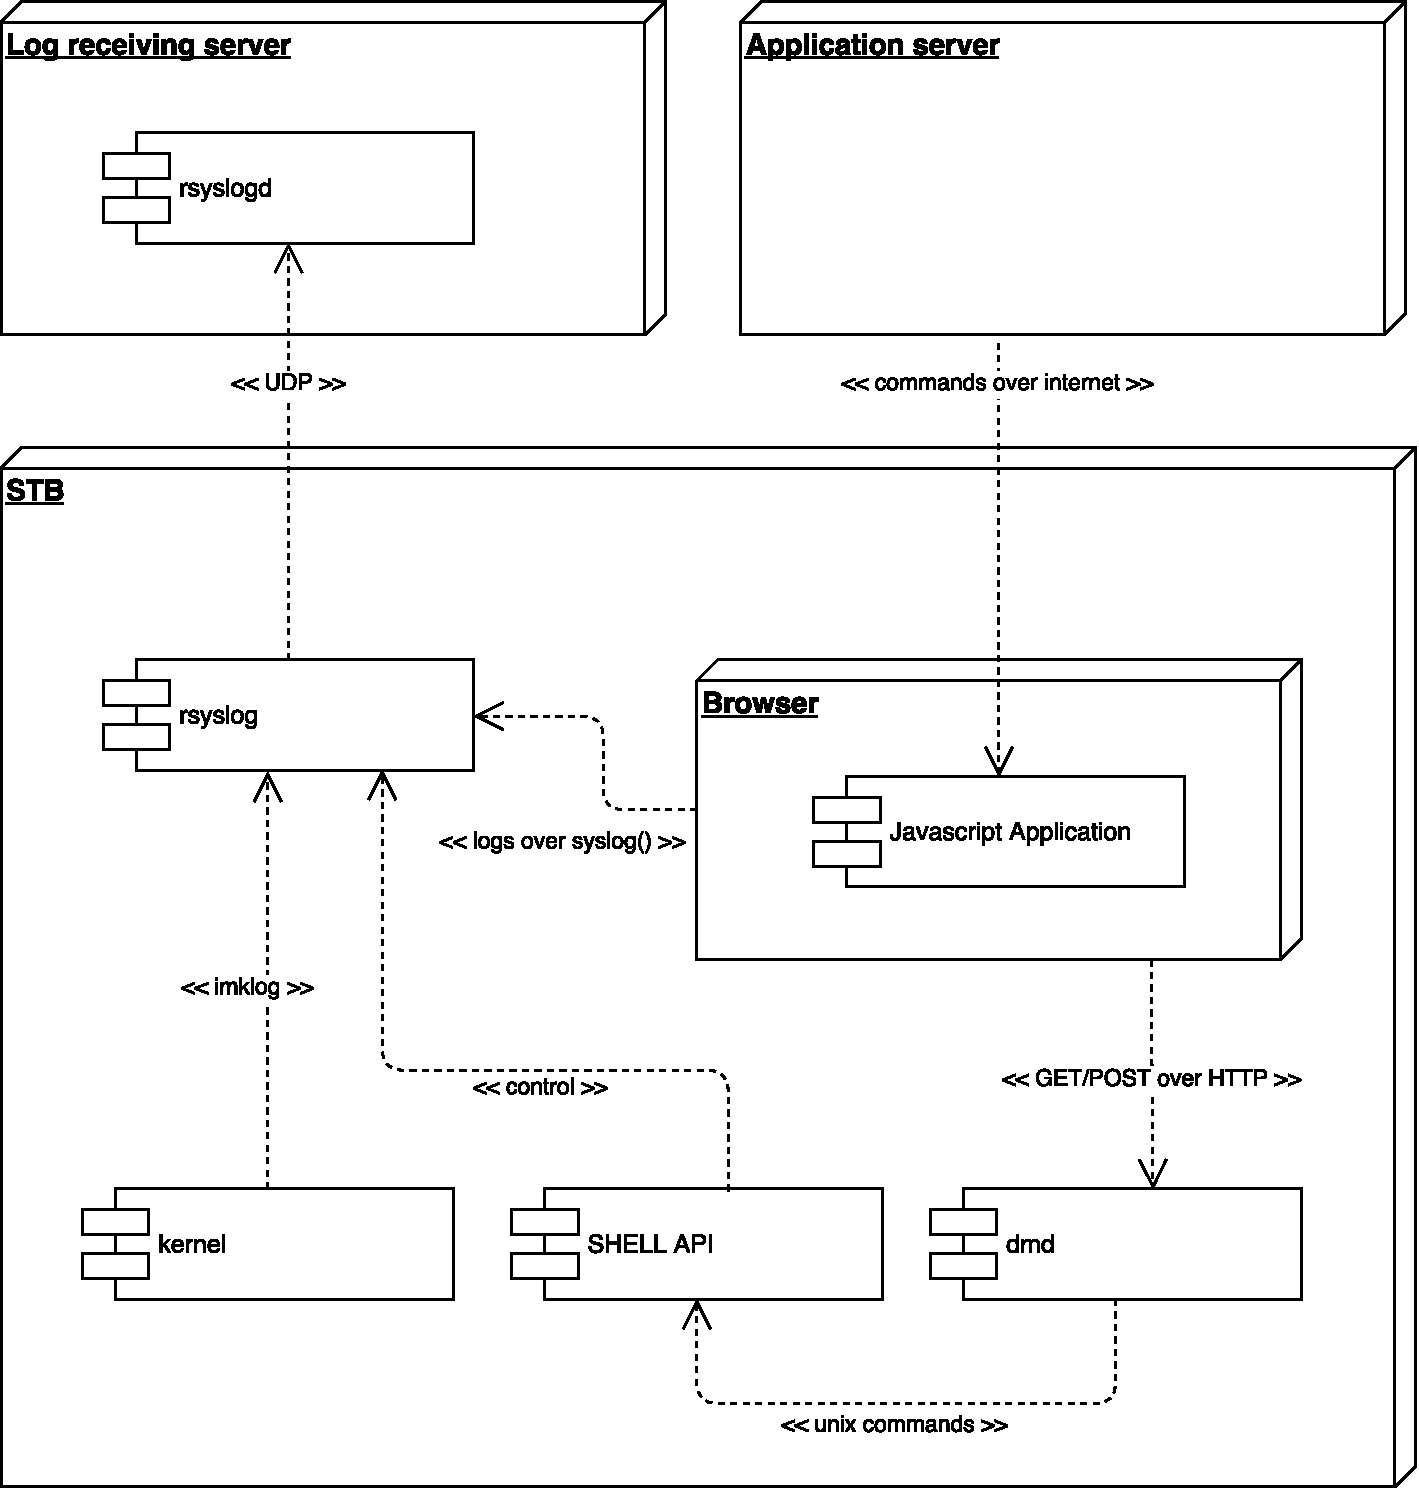
\includegraphics[scale=0.5]{images/diagram-nasazeni-noveho-reseni}
	\caption[Diagram nasazení nového řešení]{Diagram nasazení nového řešení}
\end{figure}

Prvně je nutno zvážit, zda problém řešit na straně serveru nebo set-top boxu. Vhodnou konfigurací logovacího démona na straně serveru, který by nepotřebné zprávy zavčas rozpoznal, zahodil a dále nezpracovával bychom splnili požadavek na snížení zátěže serverových disků. Přetížení sítě se takto vyřešit ale nedá a proto toto řešení zavrhuji.
Je tedy nutno problém řešit na straně set-top boxu kde původní řešení je postaveno na busy-box syslogd. Nabízí se možnost upravit fungování tím způsobem, aby se logy s nízkou severitou už na set-top boxu zahazovaly a pouze v případě potřeby bylo umožněné na dálku změnit konfiguraci démona tak, aby se povolilo logování pro logy s nastavenou danou komponentou a severitou. To vše přes SHELL-ové API.
Součástí zadání je ale i implementovat škrcení zpráv, aby nedocházelo k zahlcení linky. Takovou možnost prostý syslogd neposkytuje a je proto nutno zvážit napsání vlastního démona či nasazení jiného, vyspělejšího logovacího démona.


\section{Srovnání logovacích démonů}
V této kapitole zmíním a popíši vybrané logovací démony a v závěru kapitoly je porovnám.

\subsection{BusyBox Syslogd}
Tato logovací utilita se skládá ze dvou démonů, jmenovitě z Klogd, který zachytává logy z kernelu a předává je ke zpracování Syslogdémonu. Syslogd pak zachytává i všechny zbylé logy a dále s nimi nakládá. Má však velice omezenou funkcionalitu. Dokáže pouze logy lokálně ukládat, přeposílat je dále po síti, zahazovat duplikáty, rotovat logy v závislosti na velikosti a filtrovat zprávy podle omezených kritérií. Dokáže totiž filtrovat pouze podle typu facility a už nikoliv podle názvu komponenty, která log vygenerovala.

\subsection{Syslog-ng}
Flexibilní logovací démon zaměřený na centralizované a zabezpečené logování. Má široké možnosti nastavení a poskytuje obrovské množství funkcionalit. Takže jeho vhodným nakonfigurováním se dají snadno splnit všechny vytyčené technické požadavky až na požadavek pro možnost vzdálené změny konfigurace.
Je nutno ale zmínit, že pokročilé funkce jako například šifrování zpráv, bufferování nebo message-rate kontrola jsou dostupné pouze v komerční closed-source verzi.

\subsection{Rsyslog}
Výčet funkcionalit Rsyslogu je ještě obsáhlejší než u Syslog-ng~\cite{Rsyslog-features}. Technické požadavky se s jeho použitím tedy také dají splnit všechny, kromě vzdálené změny konfigurace. Oproti Syslog-ng je Rsyslog kompletně zdarma a open-source. Navíc není jen logovacím démonem, ale i analyzérem logů. Dokáže logy podle obsahu zprávy měnit, třídit a jinak s nimy nakládat.
Že je Rsyslog vyspělý a kvalitní program dokazuje fakt, že je defaultním logovacím démonem na spoustě linuxových distribucích, jmenovitě například v Ubuntu.
Jeho slabiny shledávám v nedostatečné dokumentaci a ve specifických případech v neefektivním analyzování logů mající za následek (obvzláště na embedded zařízení s pomalým ARM procesorem) rychlostní deficit. Jeho vývoj obstarává z velké většiny pouze jeden člověk, jeho původní tvůrce Rainer Gerhards. A v jednom člověku není snadné dovést tak rozsáhlý projekt k dokonalosti.

\subsection{Porovnání logovacích utilit}
Pouhým nasazením jakéhokoli známého logovacího démonu není možné splnit všechny vytyčené technické požadavky. V případě ponechání původního BusyBox syslogd démonu by pro splnění technických požadavků bylo nutno doimplementovat tolik funkcionalit, že by to výrazně přesahovalo rozsah bakalářské práce.
Výhodněji se jeví nasadit pokročilý logovací démon jako je Syslog-ng či Rsyslog. Oba totiž poskytují námi požadované funkcionality. Syslog-ng však většinu z nich poskytuje pouze v placené closed-source verzi a proto jsem se rozhodl pro Rsyslog.

\section{Šifrování zpráv}



\section{Komprese zpráv}
TODO


\chapter{Realizace}

\section{Sestavení a instalace Rsyslogu na STB}
 
Rsyslog není součástí SDK a tak jej bylo nutné a všechny knihovny na kterých závisí (zlib, libestr, libee, liblogging a libfastjson) zkompilovat a posléze nainstalovat na STB. K tomu bude použit systém Gu.

\subsection{Buildovací systém Gu}
Gu je buildovací systém pro linuxová embedded zařízení, který si klade za cíl zjednodušit a urychlit buildovací proces. Gu využívá balíčkovací systém pacman (převzatý z Arch Linuxu) a nástroj scratchbox2 sloužící k zjednodušení cross-kompilace. Tyto 2 nástroje jsou skryty v konzolovém přikazu \uv{gu}, kterým se celé Gu ovládá.

\subsection{PKGBUILD}
Jedná se o shellový script obsahující informace potřebné pro sestavení jednotlivých aplikací systémem Gu. Jeho syntaxe je podrobně popsána v odstavci níže.

\subsection{Sestavení a instalace aplikací}
Jako příklad zde uvádím soubor PKGBUILD pro sestavení a instalaci Rsyslogu. V podobném duchu jsou napsány i skripty pro ostatní aplikace a knihovny.
\begin{lstlisting}[style=PKGBuildStyle]
pkgname=rsyslog
pkgver=8.16.0-nangu-0.3
arch=('armv7h' 'armv7sp')
depends=('zlib' 'libestr' 'libee' 'liblogging' 'libfastjson')
source=${pkgname}-${pkgver}.tar.gz
md5sums=('SKIP')

build() {
	cd ${pkgname}
	PKG_CONFIG_PATH=/mnt/hdd_1/lib/pkgconfig
	autoreconf -fvi
	./configure --prefix=/mnt/hdd_1 \
	--disable-uuid --enable-mmsequence \
	--enable-mmsevrewrite --enable-mmdelstr
	make V=1
}

package() {
	cd ${pkgname}
	make install DESTDIR=${pkgdir}
}
\end{lstlisting}

\begin{description}
  \setlength\itemsep{-1ex}
  \item [pkgname:] Název balíčku (měl by se shodovat s názvem zdrojového archivu aplikace).
  \item [pkgver:] Verze balíčku (měla by se shodovat s verzí sestavované aplikace).
  \item [arch:] Pole specifikující architektury cílových systémů.
  \item [depends:] Pole názvů balíčků, které musí být nainstalovány před spuštěním tohoto softwaru.
  \item [source:] Seznam souborů nutných pro sestavení balíčku. Soboury mohou odkazovat na lokální úložiště, nebo na vzdálený server, v tom případě se se skript postará o jejich stažení. Komprimované soubory skript automaticky rozbalí.
  \item [md5sum:] Pole kontrolních součtů pro každý specifikovaný \uv{source}.
  \item [build():] Nepovinná funkce obsahující příkazy vedoucí ke konfiguraci a sestavení aplikace.
  \item [package():] Povinná funkce instalující soubory. Funkce je spouštěna až po exekuci ostatních nepovinných funkcí.
  \item [pkgdir:] Proměnná obsahující umístění kořenového adresáře instalované aplikace.
\end{description}

Po vstoupení do adresáře obsahujícím zdrojové kódy aplikace a skript PKGBUILD stačí zadat příkaz \uv{gu build}, čímž se uvede do chodu celý skript. Nejdříve se inicializují proměnné, posléze se vykoná funkce build() a nakonec package(), čímž by měl (pokud nedojde k žádné chybě) vzniknout v umístění \uv{pkdir} balíček s přeloženou aplikací.
Příkazem \uv{gu install <název-vzniklého-balíčku.tar.xz>} nainstalujeme balíček do SDK.

\section{Konfigurace Rsyslogu}
Rsyslog se řídí podle pravidel specifikovaných v konfiguračním souboru /etc/rsyslog.conf. Za použití tzv. compatibility módu~\cite{Rsyslog-comp-mode} podporuje syntaxi známou z dříve na linuxu hojně užívaného démonu sysklogd. Níže je uveden příklad konfiguračního souboru syslog.conf~\cite{Syslog-conf} pro sysklogd. Na levo je možno specifikovat kritéria pro filtraci zpráv podle jejich severity a facility. Na pravo je pak umístění, kam zprávy odesílat.

\begin{lstlisting}[style=RainerScriptStyle]
*.=crit;kern.none            /var/adm/critical
kern.*                       /var/adm/kernel
kern.crit                    @finlandia
kern.crit                    /dev/console
kern.info;kern.!err          /var/adm/kernel-info
\end{lstlisting}

Díky této podpoře je možno velice snadno migrovat z Syslogd na Rsyslogd.
Pro využití i jiných než základních funkcí Rsyslogu, je nutno k nakonfigurování pravidel použít syntaxi jazyku Rainerscript.

\subsection{Rainerscript}
Rainerscript~\cite{RainerScript} je skriptovací jazyk navržený ke správě síťových událostí (převážně nakládání se syslog zprávami) a dále ke konfiguraci softwaru, pro který je používán.
Tento jazyk je totiž teoreticky použitelný v ruzných typech softwarů, nicméně v době psaní této práce byl vyvíjen a reálně pužíván pouze v Rsyslogu.

Jedná se o netypový jazyk, který poskytuje podporu regulárních výrazů~\cite{RainerScriptPropertyReplacer} a má nadefinované užitečné funkce především pro práci s textovými řetězci.
Podrobnosti jsou k nalezení v dokumentu s formální definicí jazyka~\cite{RainerScriptFormalDefinition}.

\subsection{rsyslog.conf}
Níže je uvedena ukázka RainerScript konfiguračního souboru, kde jsou předvedeny základní konstrukce používané při jeho tvorbě.

\begin{lstlisting}[style=RainerScriptSimpleStyle]
module(load="NazevModulu")
\end{lstlisting}
Na začátku souboru je možné načíst různé moduly, poskytující doplňující funkcionality. Příkladem může být modul imklog čtoucí zprávy z kernelu nebo omfwd umoňující posílat zprávy zkrze UDP nebo TCP protokoly. Je nutno poznamenat, že některé moduly nejsou defaultně kompilovány spolu s rsyslogem a je proto nutno přidat příkazu compile parametr $-$$-$enable$-$<název\_modulu>.

\begin{lstlisting}[style=RainerScriptSimpleStyle]
set $!Promenna="hodnota";
unset $!Promenna;
\end{lstlisting}
Pomocí klíčovích slov set a unset je možné deklarovat a rušit proměnné. Ty začínají znaky \$! a příkaz je nutno ukončit středníkem.

\begin{lstlisting}[style=RainerScriptSimpleStyle]
template(name="nazev-sablony" type="string" string="<%pri%>%TIMESTAMP:::date-rfc3164% %$!macaddr% %syslogtag% id=%$!counter%%msg%\n"
	)
\end{lstlisting}
Šablony definují podobu zpráv. Do proměnné string lze vložit libovolné textové řetězce. Proměnná mezi dvojicí znaků procento je nahrazena jejich obsahem. Použity mohou být vlastní lokální proměnné a nebo tzv. replacement proměnné, vztahující se typicky k syslog zprávě, ve kterých je uložena např. severita nebo například čas odeslání. Nejdůležitější je proměnná msg, kde je uložen text zprávy.

\begin{lstlisting}[style=RainerScriptSimpleStyle]
action(template="nazev-sablony" type="omfwd" Target="192.168.1.10" Port="5514" Protocol="udp" )
\end{lstlisting}

Pomocí akcí se volají jednotlivé moduly. Ty mohou mít různé parametry, které upravují jeho chování. V ukázce výše se volá modul omfwd sloužící k posílání zpráv skrze síť. Parametry specifikují konkrétní IP a port sítě, typ protokolu a název šablony, která upravuje formát zpráv.

\begin{lstlisting}[style=RainerScriptSimpleStyle]
if $programname == 'solid' and $syslogseverity > 5
then {
	#nejaka akce
	stop
}
\end{lstlisting}
	
Použití podmínky if je zřejmé z ukázky výše. V podmínce if se obvykle volají různé akce.

Veškerý text za symbolem \uv{\#} až do konce řádky je považován za komentář.
\\
\\
Nyní po obeznámení se základní syntaxí Rainerscriptu je možno popsat fungování zachytávání jednotlivých zpráv. Ty imaginárně putují skrze kód rsyslog.conf odshora dolů, kde prochází skrze podmínky a akce (které je eventuelně upravují nebo např. zapisují do souborů) a to až do doby, než narazí na klíčové slovo stop nebo na poslední řádek souboru.

\subsubsection*{Rsyslog queues}

\begin{figure}[ht]
	\centering
	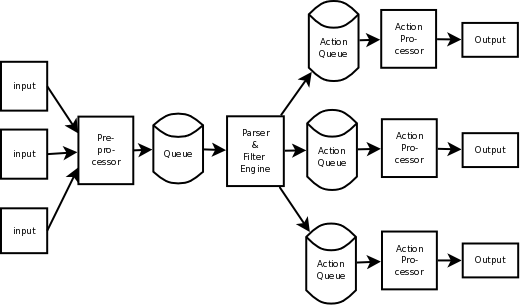
\includegraphics[scale=0.4]{images/rsyslog-queues}
	\caption[Rsyslog queues]{Rsyslog queues~\cite{RsyslogQueues}}
\end{figure}

Princip fungování front v Rsyslogu je znázorněn na obrázku níže. Zprávy (ať už lokální nebo ze vzdáleného zdroje putující do Rsyslogu např. skrze UDP) vstupují do Rsyslogu  na obrázku zleva, kde jsou předzpracovány a putují do Main Queue. V dalším kroku jsou zprávy tříděny podle pravidel specifikovaných v rsyslog.conf a putují do jednotlivých action queues. Následně proběhne finální zpracování zpráv a opouštějí rsyslog skrze výstupní modul ať už zápisem do lokálního souboru nebo např. předáním jinému procesu.

Všechny zprávy tedy projdou nejprve skrze Main Queue a poté skrze libovolný počet Action Queues. Je nutno zmínit, že každá akce obsahuje vlastní frontu, ve které zprávy čekají na zpracování. V případě, že v akci žádnou frontu nepotřebujeme, stačí nastavit jako Action Queue mód Direct mode.

Existují totiž čtyři módy front. Speciálním (a výchozím) je Direct mode. Direct Queues ve skutečnosti nejsou frontami. Neobsahují totiž žádný buffer a zprávy rovnou přeposílají dál. Vhodné jsou například při zápisu logů do souboru na lokální úložiště.

Druhým typem jsou In-Memory Queues, které udržují zprávy v na operční paměti uloženém bufferu. Výhodou je vysoká rychlost a nevýhodou zase hrozba ztráty dat v případě neočekávaného pádu systému.
Existují dva podtypy In-Memory front. Můžou být implementovány formou spojového seznamu (LinkedList queue) nebo za použití pole ukazatelů na prvky fronty (FixedArray) s předem pevně určeným počtem prvků. FixedArray mode je nejrychlejší ze všech módů a je vhodný pro případy, kdy očekáváme pouze malý počet prvků ve frontě. LinkedList queue dynamicky alokuje místo v paměti pro každou zprávu.
Obecně se doporučuje použití implementace postavené na spojovém seznamu, jelikož výkonostní propad oproti fixnímu poly je zanedbatelný, zato úspora paměťového místa může být značná.
 
Třetí typ front představují Disk Queues, které jak z názvu vyplývá bufferují na disk. Využití najdou v případech kdy si žádáme vysokou soplehlivost. Jejich nevýhodou je pomalost limitovaná rychlostí perzistentních úložišť.

Disk-Assisted Memory Queues fungují stejně jako In-Memory Queues a navíc v případě potřeby (kterou může být nedostatek místa nebo nutnost uložení zpráv z bufferu z nutnosti zálohy zpráv z perzistentní paměti před vypnutím systému) dokáží obsah fronty nebo její část přesunout na disk. Používají chytrý algoritmus, který při malém vytížení vůbec nepoužívá disk queues. V případě vyčerpání kapacity In-Memory fronty se algoritmus postará o přesun části zpráv do diskové fronty.

\subsubsection*{Rate-limiting za použití Rsyslog queues}
Původní řešení trápil neduh, kdy k vyprázdnění bufferu docházelo až s nově příchozí zprávou, což mělo za následek, že v případě zaplněného bufferu a následující delší odmlky nově příchozích zpráv mohlo dojit k velkému zpoždení odeslání zpráv v ten moment uložených v bufferu. Tento problém se nasazením Rsyslogu a použitím jeho sofistikovaných front vyřeší.
V této kapitole je popsána implementace fronty, která má za cíl škrtit tok odchozích zpráv podle stejných kritéri, jak tomu bylo původně.
Původní řešení bylo postavené na syslogd démonu doplněné o hardcodovaný rate-limiting zpráv a fungovalo následovně. Všechny příchozí zprávy putovaly do fronty o fixní velikosti 128 kB. V případě, kdy tok odchozích zpráv překročil 150 kbit/s nebo počet zpráv ve frontě přesáhl 800 byly nově příchozí zprávy zahozeny.
Rsyslog neumožňuje nastavení maximálního toku sítě, avšak poskytuje možnost nastavit pro frontu tyto parametry:
\begin{description}
  \setlength\itemsep{-1ex}
  \item [queue.size:] Maximální počet zpráv ve frontě.
  \item [queue.dequeuebatchsize:] Maximální počet zpráv vystupujících z fronty v jeden okamžik.
  \item [queue.dequeueslowdown:] Zpoždění (v $\mu$s) mezi odesíláním jednotlivých zpráv (v případě queue.dequeuebatchsize>1 bloků zpráv).
\end{description}
Queue.size tedy nastavíme stejně na 800 zpráv.
Pro dequeuebatchsize jsem zvolil hodnotu 5 - TODO, proč vlastně zrovna 5..
Nyní je třeba zjistit parametry pro dequeueslowdown. Z měření bylo zjištěno, že průměrná velikost UDP paketu se zprávou ze STB má 150~B. Pomocí níže zobrazených vzroců jsme snadno spočetli požadované zpoždění v mikrosekundách, aby zátěž linky nepřekročila 150 kbit/s.
\begin{description}
  \item $počet~zpráv=\frac{bandwith}{velikost~paketu}=\frac{150~*~1~000~[b]}{8~*~150~[b]}=125$
  \item $zpoždění=\frac{1~sekunda}{počet~zpráv}=\frac{1~000~000}{125}*dq.~slowdown~=~8~000~*~5~=~40~000~[\mu$$s]$
\end{description}
Ještě zbývá zvolit typ fronty, kde kvůli důrazu na rychlost byla zvolena implementace založená na spojovém seznamu.
Výsledný kód pro akci s In-memory frontou s nastaveným rate-limitingem vypadá následovně:
\begin{lstlisting}[style=RainerScriptSimpleStyle]
action(type="omfwd" target="192.168.1.10" port="5514" queue.size="800" queue.dequeueslowdown="40000" queue.dequeuebatchsize="5" queue.type="LinkedList" )
\end{lstlisting}


\subsection{Razítkování zpráv}
Požadavkem zadavatele bylo značit všechny zprávy vzestupnou řadou čísel kvůli rozpoznání případného výpadku některých zpráv.
Byl pro to použit modul mmsequence~\cite{RsyslogMmsequence}, který byl nastaven jako je ukázáno v kódu níže.
\begin{lstlisting}[style=RainerScriptSimpleStyle]
module(load="mmsequence")
action(	type="mmsequence"
		from="1"
		to="1048576" # 2^20
		var="$!counter" )
\end{lstlisting}
Proměnné \uv{\$!counter} je tak přiřazeno číslo \uv{1} a s každou další příchozí zprávou se číslo zvýší o \uv{1} dokud nenarazí na maximální hodnotu specifikovanou parametrem \uv{to}, kdy je číslo vyresetováno na původní hodnotu \uv{1}.
Tato proměnná je následně používána v šablonách a je tak připojena k tělu každé zprávy.

\subsection{Formát logů}
Požadavkem zadavatele je, aby zprávy měli identický formát, jako tomu bylo u původního řešení. Důvodem je, že logy ze STB sbíra vzdálený server, který očekává daný formát.
\\
\\
Vzor zprávy:
\begin{lstlisting}[style=RainerScriptSimpleStyle]
May  1 19:04:54 cc-b8-f1-04-17-89 solid: id=8853 Player Time [00:06:56.96]
\end{lstlisting}
Formát:
\begin{lstlisting}[style=RainerScriptSimpleStyle]
<PRI><RFC3164 date> <STB mac address> <component>: <id=NUM>  <message>
\end{lstlisting}

Můžeme si povšimnout, že vzorová zpráva začíná datumem a přitom formát zprávy obsahuje na prvním místě číslo PRI a až poté následuje datum. Hodnota PRI totiž není viditelná a slouží logovacímu démonu, který z ní dokáže vypočítat severity a facility zprávy.

\subsubsection{Šablony}
Šablony specifikují výslednou podobu zpráv a jejich použití je intuitivní, proto rovnou předvedu hotovou implementaci, která splňuje požavky pro formát.

\subsubsection*{Implementace šablony}
Základní šablona pro zprávy lokálně ukládané na STB:
\begin{lstlisting}[style=RainerScriptSimpleStyle]
template( name="local-template" type="string" string="%TIMESTAMP:::date-rfc3164% %\$!macaddr% %syslogtag% id=%\$!counter%%msg%\n" )
\end{lstlisting}

\begin{description}
  \setlength\itemsep{-1ex}
  \item [name:] Název šablony, který sloužící jako identifikátor pro jednotlivé akce.
  \item [type:] Definuje typ šablony, které umožňují různé způsoby jak specifikovat obsah šablony. V této ukázce je zvolen styl string.
  \item [string:] Tento parametr je možno definovat jen v případě zvolení typu šablony \uv{string}. Jeho obsahem pak jsou konstatní textové řetězce a proměné, které jsou vměstnány mezi dvojice znaků procento.
\end{description}

\section{Rsyslog moduly}
Rsyslog poskytuje podporu tzv. modulů, které mohou zásadně rozšiřovat jeho funkcionalitu. Tyto moduly jsou obvykle napsány v jednom C souboru. Pro jejich zprovoznění je třeba náležitě upravit Makefile a zkompilovat Rsyslog se zapnutou jejich podprou.

Moduly se dělí na 6 základních kategorií, zde zmíním 3 nejpoužívanější:

\begin{description}
  \item [Output Modules:] Výstupní moduly umožňují posílat zprávy na různé cíle. Je tak možno implementovat například modul, který dokáže odesílat zprávy do nějaké exotické databáze, kterou Rsyslog v základu nezná. Jako příklad výstupního modulu zmíním ommail, což je modul sloužící k posílání zpráv skrze mail.
  \item [Input Modules:] Vstupní moduly jak název napovídá umožňují přijímat zprávy z různých zdrojů. Hojně používaný je imklog sbírající zprávy z linuxového jádra nebo imudp přijímající zprávy skrze UDP protokol.
  \item [Message Modification Modules:] Moduly, které modifikují obsah zprávy. Jako příklad uvedu v této práci použitý modul mmsequence, který generuje podle zadaných kritérií číselné řady.
\end{description}


V této práci byly naprogramovány dva moduly, oba z kategorie Message Modification Modules.

\subsection{Modul mmdelstr}
Tento modul slouží ke smazání zadaného podřetězce z těla zprávy.
\\
\\
Použití:
\begin{lstlisting}[style=RainerScriptSimpleStyle]
module(load="mmdelstr") 
action(type="mmdelstr" stringtobedeleted="Some string")
\end{lstlisting}

Modul má pouze jeden parametr \uv{stringtobedeleted}, kterým se specifikuje podřetězec, který má být smazán. V případě neexistence takového podřetězce, zůstává zpráva netknutá. V případě výskytu vícero takových podřetězců, je smazán pouze první.

\subsection{Modul mmsevrewrite}
Mmsevrewrite dokáže měnit severitu zadané zprávy. Rsyslog v základu tuto funkcionalitu neumožňuje, protože se jedná o vzácný požadavek. Modul je použit v této práci pro konverzi zpráv pocházejících z aplikace používající s Rsyslogem jinak nekompatibilní množinu severit.
\\
\\
Použití:
\begin{lstlisting}[style=RainerScriptSimpleStyle]
module(load="mmsevrewrite")
action(type="mmsevrewrite" severity="debug")
\end{lstlisting}

Modul obsahuje pouze jeden parametr \uv{severity}, kterým se určuje nová severita zprávy. V případě zadání neplatné severity Rsyslog zaloguje chybovou hlášku a upravovaná zpráva zůstane v původním stavu.

\subsection{Postprocessing zpráv}
Zadavatel si přeje vytvoření ukázek pravidel pro RainerScript, které budou sloužit jako vzor, podle kterých si sám v budoucnu vytvoří sadu vlastních pravidel.

\subsubsection{Zahazování zpráv podle typu komponenty}
Pravidlo, které rozpozná zprávy podle zadané komponenty a obsahu zprávy a ty následně zahodí.
\\
\\
Implementace pravidla:
\begin{lstlisting}[style=RainerScriptStyle]
if $programname == 'solid' and \
$msg contains "Player_GetState" then
{	
	stop
}
\end{lstlisting}
Pokud zpráva pochází z komponenty \uv{solid} a obsahuje zmíněný podřetězec, klíčové slovo stop okamžitě zahodí v ten moment zpracovávanou zprávu.
\\
\subsubsection{Převod severit}
Aplikace na STB používají pro logování jinou množinu severit, než s jakými pracuje Rsyslog. Zadavatel proto požaduje změnit severity zpráv podle následující tabulky.

\begin{table}[H]
\centering
	\caption{Převodní tabulka severit}	\begin{tabular}{|l|l|}\hline
		Portal		& Syslog			\tabularnewline \hline \hline
		ERROR		& ERR			\tabularnewline \hline
		WARN		& WARN			\tabularnewline \hline
		INFO		& NOTICE			\tabularnewline \hline
		DEBUG		& INFO			\tabularnewline \hline
		TRACE		& DEBUG			\tabularnewline \hline
	\end{tabular}
\end{table}

Implementace pravidla:
\begin{lstlisting}[style=RainerScriptStyle]
if $msg contains "mTRACE: " then
{
	action(type="mmsevrewrite" severity="debug")
}
else if $msg contains "mDEBUG: " then
{
	action(type="mmsevrewrite" severity="info")
}
\end{lstlisting}
Zprávy obsahující nesprávně nastavené severity je možno opravit podle výše zmíněného pravidla. Bylo totiž vypozorováno, že ony postižené zprávy obsahují podřetězec ve formátu \uv{m<SEVERITY>: }. Stačí pak na danou zprávu zavolat akci mmsevrewrite s parametrem severity vyplněným podle převodní tabulky severit.

\subsubsection{Smazání podřetězce z těla syslog zprávy}
Zprávám pocházejícím z komponenty solid je třeba smazat zadaný podřetězec.
\\
\\
Implementace pravidla:
\begin{lstlisting}[style=RainerScriptStyle]
if $programname == 'solid' and $msg contains
		":[notificationFromPlayer]: INFO: " then
{
	action(type="mmdelstr" \ 
	stringtobedeleted=":[notificationFromPlayer]: INFO: ")
}
\end{lstlisting}


\section{Vzdálená konfigurace}
Požadavkem zadavatele je umožnit změnu nastavení maximální povolené severity jednotlivých komponent. Rsyslog neumožňuje změnu konfiguračního souboru za jeho běhu a proto je nutno implementovat API, které umožní přenastavení konfiguračního souboru a jeho znovunačtení (restartováním Rsyslogu).
Změny tímto skriptem způsobebé musí být zachovány i po restartu STB.

\subsection{Návrh API}
Skript musí umět nastavi konfiguraci souboru rsyslog.conf tak, aby v případě rozpoznání zprávy od určité komponenty spolu s nastavenou severitou vyšší, než je povolená, danou zprávu zahodil. 
Musí tedy umět v daném skriptu nalézt část kódu, kde se zpracovává zadaná komponenta a tuto část kódu vhodně upravit.

V úvahu připadaly 2 různé přístupy. Je možné při každém zavolání scriptu generovat celý nový konfigurační soubor a nebo parsovat stávající soubor a jeho část pomocí skriptu měnit.
Výhodou prvního způsobu je, že nehrozí nechtěné přepsání jiných čásí skriptu, než bylo zamýšleno. Nevýhodou je složitější implementace z důvodu nutnosti pří generování nového skriptu zohledňovat předchozí nastavení skritpu. Tedy by bylo nutno z původního skriptu extrahovat nastavení jednotlivých komponent a to zkombinovat s novým nastavením.
Rozhodl jsem se proto pro 2. způsob řešení s tím, že zadavatel bude poučen o nutnosti dodržovat určité zásady při měnění konfiguračního souboru, aby nemohlo dojít k neočekávanému chování.

\subsection{Výběr implementačních nástrojů}
Jazyky jako Perl nebo Python se jeví jako ideální pro napsánání skriptu na zpracování textu. Tyto ani jiné podobné jazyky ovšem nejsou součástí SDK a zadavatel si nepřeje jejich instalaci z důvodu omezené paměti nevalného výkonu embedded zařízení. Nezbýva než se spokojit s na STB přítomnou minimalisticou BusyBox implementací SHELLu nesoucí název ASH. Ta sice neposkytuje tak elegantní syntaxi a neposkytuje tolik rozšířených funkcionalit jako moderní SHELL-ové jazyky typu BASH, ale i přesto se s její pomocí a základních UNIXových programů jako například GREP je možno API naprogramovat.

\subsection{Rozhraní skriptu}
První možností je napsat API ve formě scriptu, který přijímá jednotlivé názvy komponent a jim příslušící maximální povolenou severitu jako parametry.

\begin{lstlisting}[style=RainerScriptSimpleStyle]
set_log_verbosity.sh [component] [severity] ...
\end{lstlisting}

Jako druhá možnost připadá v úvahu skript, který čte seznam jednotlivých komponent a maximálních povolených severit ze souboru, který má následující formát:

\begin{lstlisting}[style=RainerScriptSimpleStyle]
component1  = DEBUG
componentXY = INFO
...
DEFAULT     = INFO
\end{lstlisting}

Se zadavatelem jsme se shodli, že se lépe jeví první způsob pro jeho jednoduší a rycheljší obsluhu a navíc s jeho použitím pro zadavatele odpadá starost o další konfigurační soubor.

\subsection{Implementace API}
Skript na vstupu očekává sudý počet parametrů, kde každý sudý parametr je název komponenty a liché parametry slouží pro definování severit pomocí jejich číselných hodnot.
Skript vyhledá v konfiguračním souboru rsyslog.conf řádek s danou komponentou a přenastaví maximální povolenou severitu. Skript kontrolojue správnost vstupních parametrů pro zabránení neočekávaného chování programu.

\chapter{Testování}
TODO úvod do testování. Co, jak, proč..

Pro účely testování byl použit Apple Macbook 13 (dále jen PC) s následující konfigurací.
\subsection*{kofigurace PC}
\begin{description}
\setlength\itemsep{-1ex}
  \item [CPU:] 2,7 GHz Intel Core i5
  \item [RAM:] 8GB DDR3
  \item [OS:] OS X 10.11.4
\end{description}

\subsection*{Testovací syslog server}
Pro účely testování byla na Wifi routeru Huawei HG622u nakonfigurována lokální síť (jakožto simulace reálných serverů zadavatele). Na výše zmíněném PC, byl nakonfigurován logovací démon syslog-ng pro sběr logů od STB pomocí definování naslouchání na daném UDP portu. PC je tedy v testech použito jakožto syslog server.

\subsection{Test zahlcení zprávami za běžného provozu}
 V tomto testu srovnávám vytížení linky nového a starého logovacího řešení při běžném provozu STB. 

\begin{figure}[H]
	\centering
	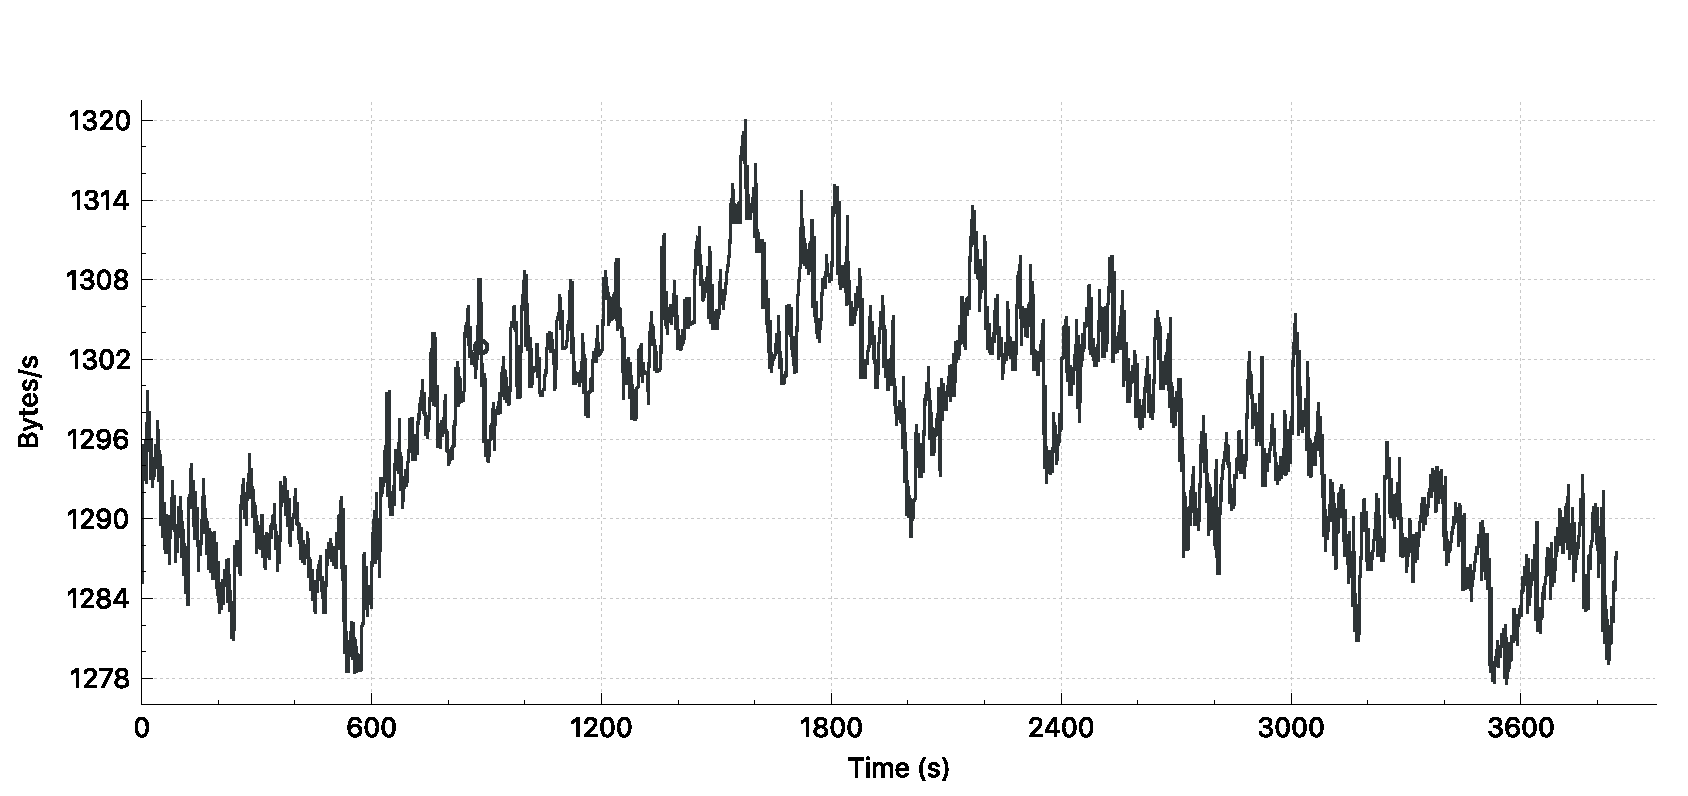
\includegraphics[scale=0.44]{images/test-1h-syslogd-default}
	\caption[Syslogd]{Syslogd}
\end{figure}

\begin{figure}[H]
	\centering
	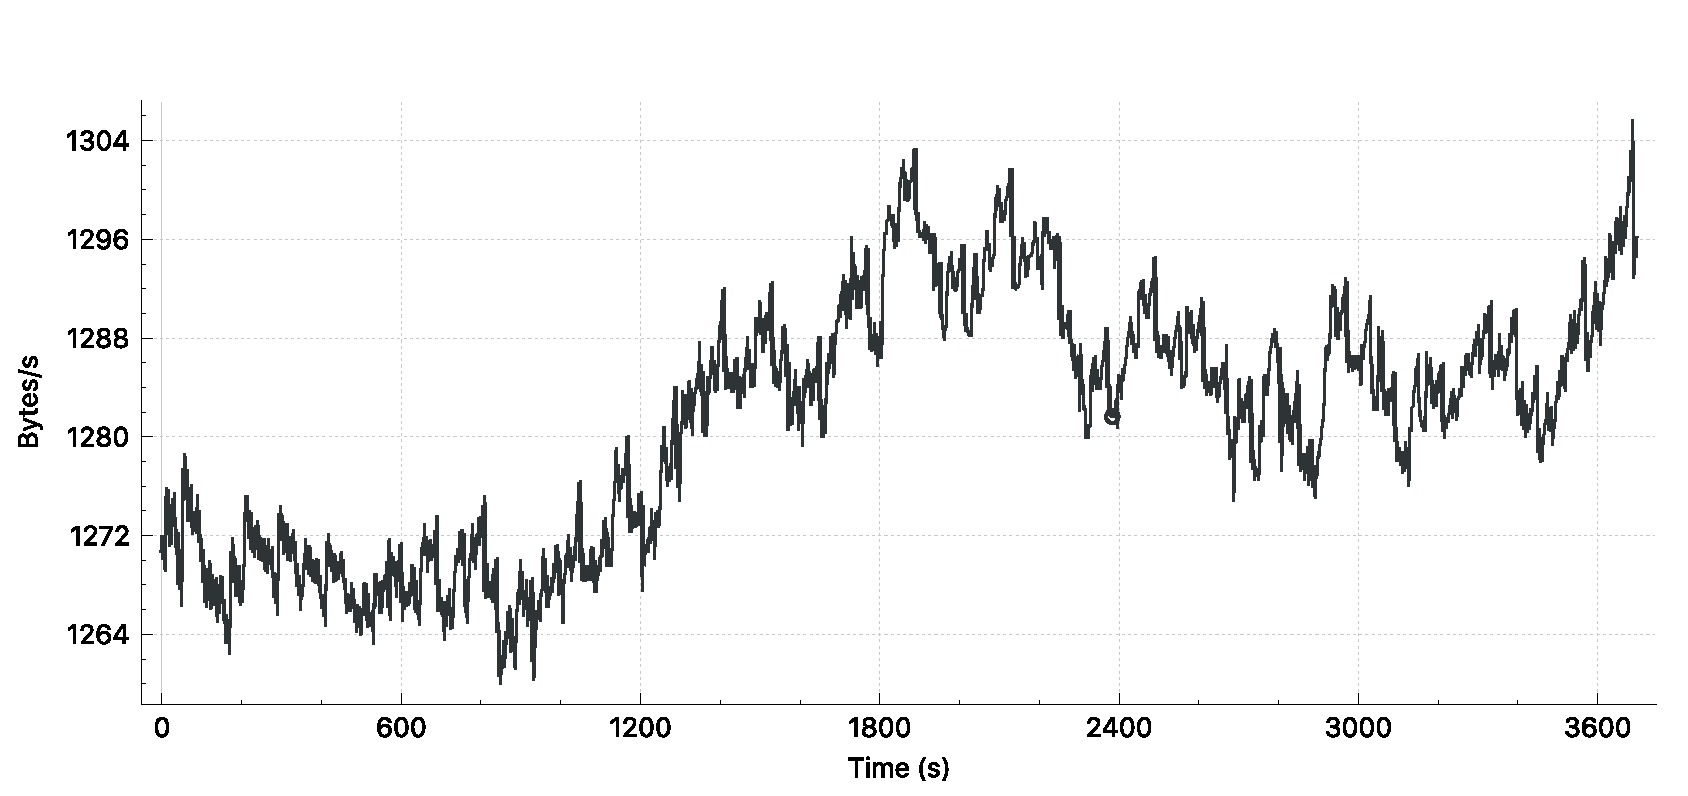
\includegraphics[scale=0.44]{images/test-1h-rsys-default}
	\caption[Rsyslogd]{Rsyslogd}
\end{figure}

\begin{figure}[H]
	\centering
	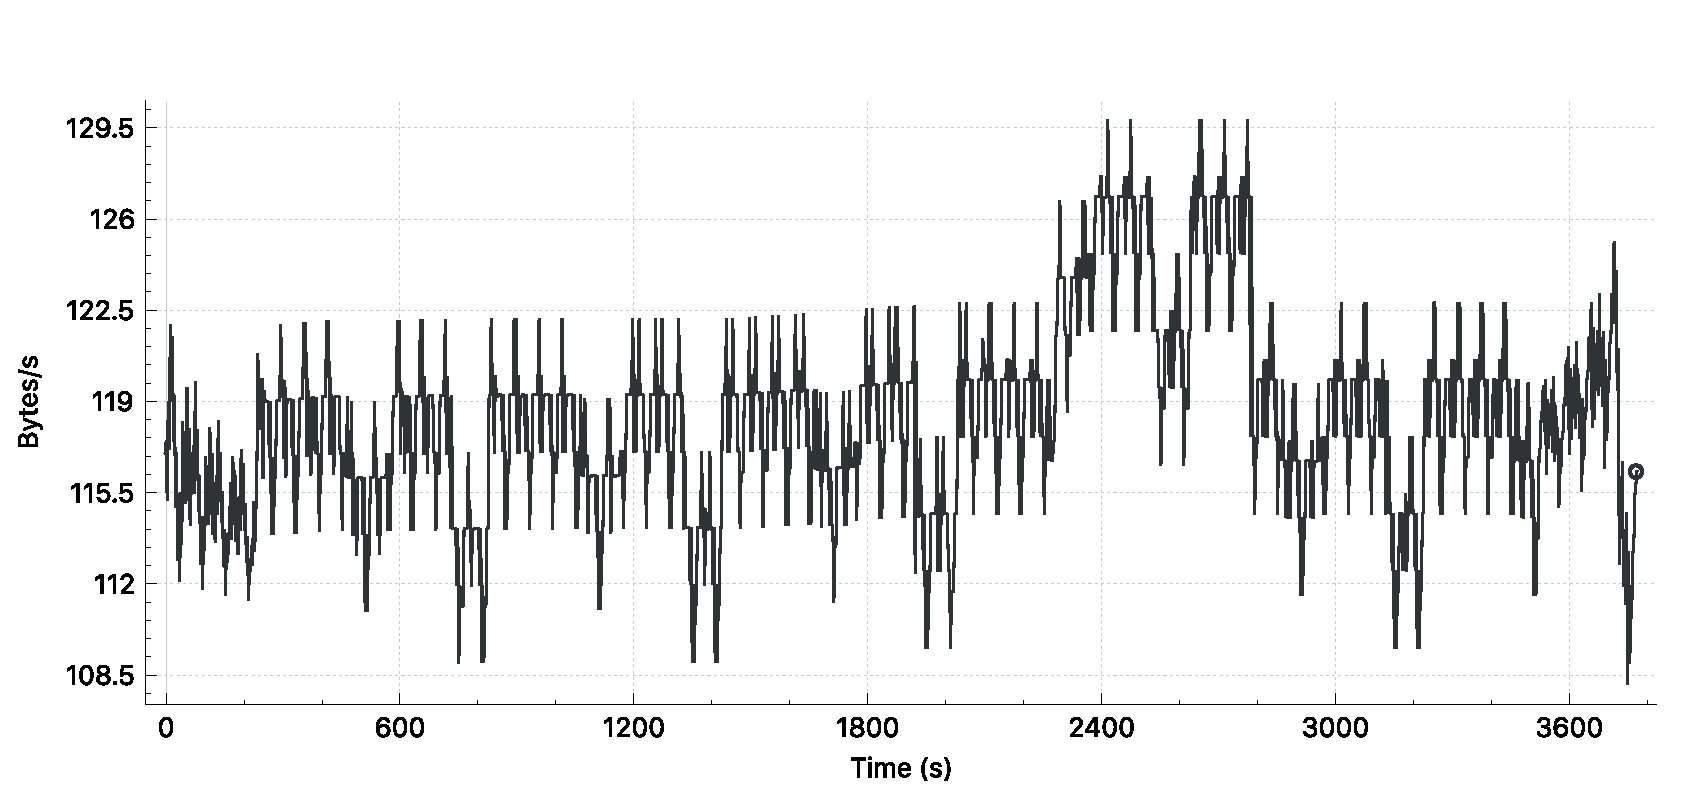
\includegraphics[scale=0.44]{images/test-1h-rsys-solidoff}
	\caption[Rsyslogd - aplikace Solid vypnuta]{Rsyslogd - aplikace Solid vypnuta}
\end{figure}

\subsection*{Zhodnocení}
Jak je vidět z prvních dvou grafů, nové řešení postavené na rsyslogd přijíma méně logů. Je to způsobeno jeho konfigurací, v níž je nastaveno pravidlo (viz kapitola 4.3.3.1), kterým se zahazují určité nepotřebné zprávy. Na STB totiž běží aplikace, již zadavatel nemá možnost upravit, která loguje mimo jiné i nepotřebné zprávy. V původním řešením podobné pravidlo nebylo možné jakkoliv nastavit.
Dle Wiresharku tak nové řešení v průměru přijíma 8,6 paketů za sekundu oproti 9 paketům za sekundu v původním řešení.

V třetím grafu je pro zajímavost znázorněno zahlcení linky při použití nového řešení po zakázání zpráv od komponenty solid.
Chci tím demonstrovat, že zadavatel má v novém řešení možnost si upravit filtrování zpráv podle různých kritérií a může tak razantně snížit zahlcení sítě.

\section{Test škrcení zpráv}
V tomto testu se ověřuje funkčnost rate-limitingu.
K tomu je použit skript generující obrovské množství logů v krátkém časovém intervalu. Funkce gen\_messages() pomocí příkazu logger posíla 1000 zpráv syslog démonu. Tato funkce je navíc volána v deseti paralelních instancích.

\begin{lstlisting}[style=AshStyle]
#!/bin/sh
gen_messages() {
	for i in $(seq 1000); do
		logger 	"Zprava o 100B..."
	done
}
for i in $(seq 10); do
	gen_messages &
done
\end{lstlisting}

\subsection*{}
\begin{figure}[H]
	\centering
	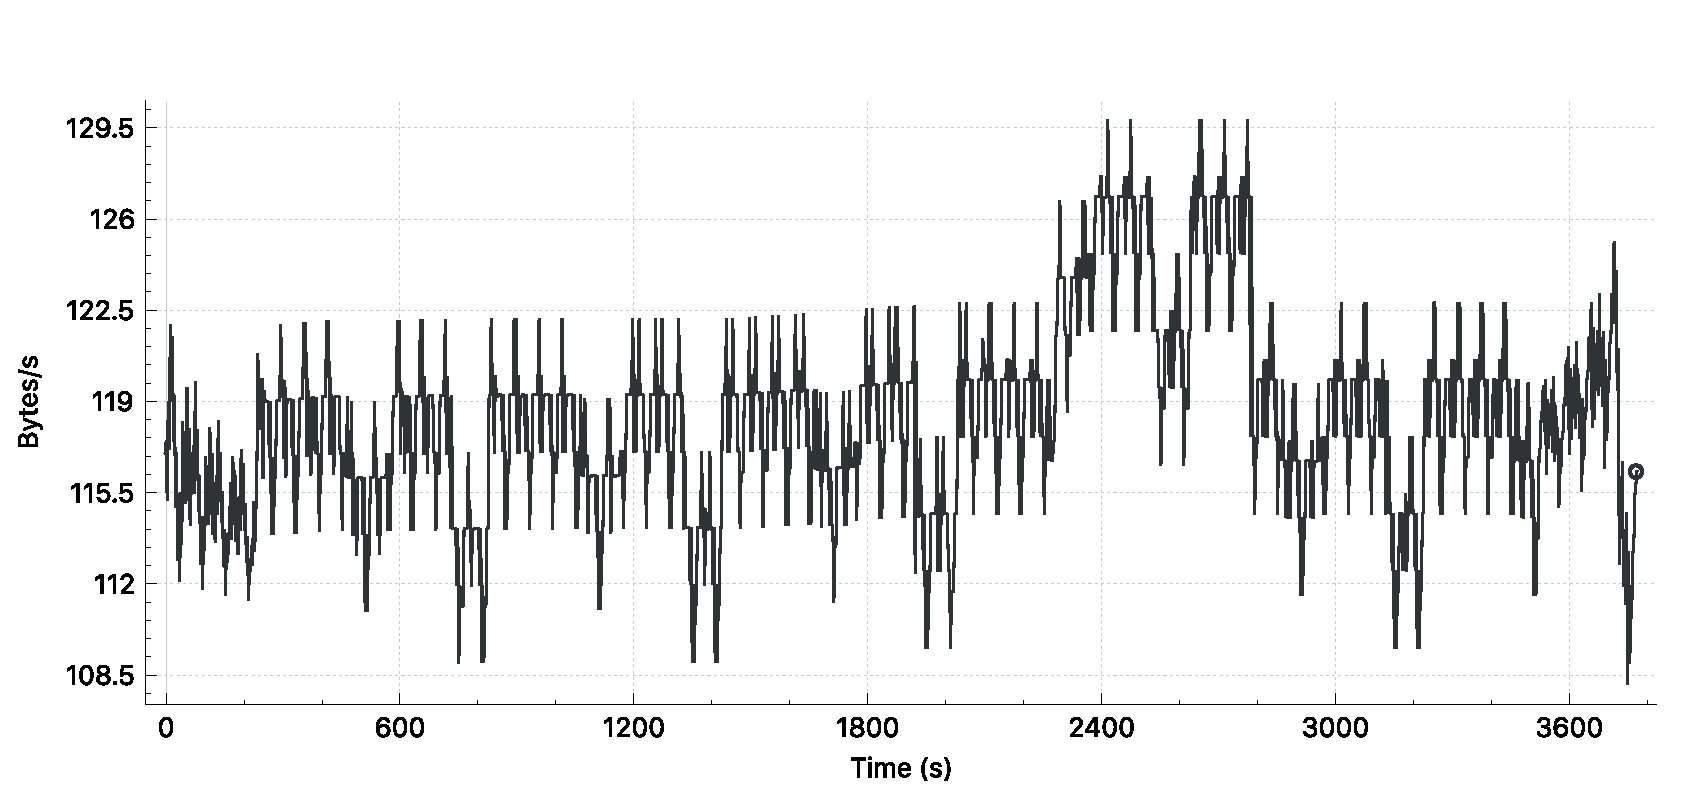
\includegraphics[scale=0.44]{images/test-1h-rsys-solidoff}
	\caption[Vytížení bez zapnutého škrcení zpráv]{Vytížení bez zapnutého škrcení zpráv}
\end{figure}

\begin{figure}[H]
	\centering
	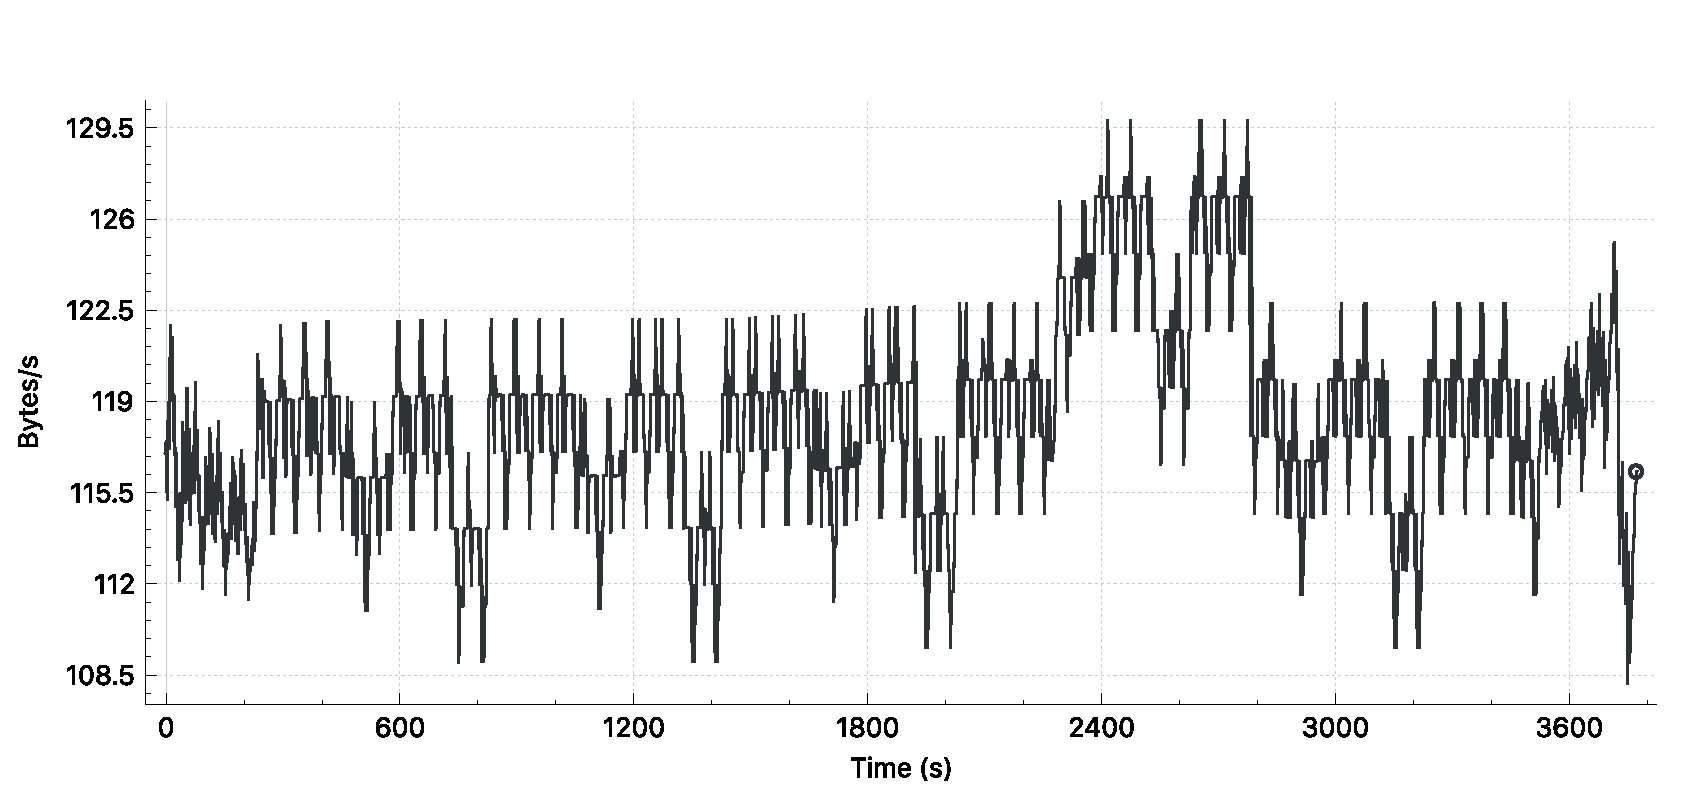
\includegraphics[scale=0.44]{images/test-1h-rsys-solidoff}
	\caption[Vytížení na původním syslogd]{Vytížení na původním syslogd}
\end{figure}

\begin{figure}[H]
	\centering
	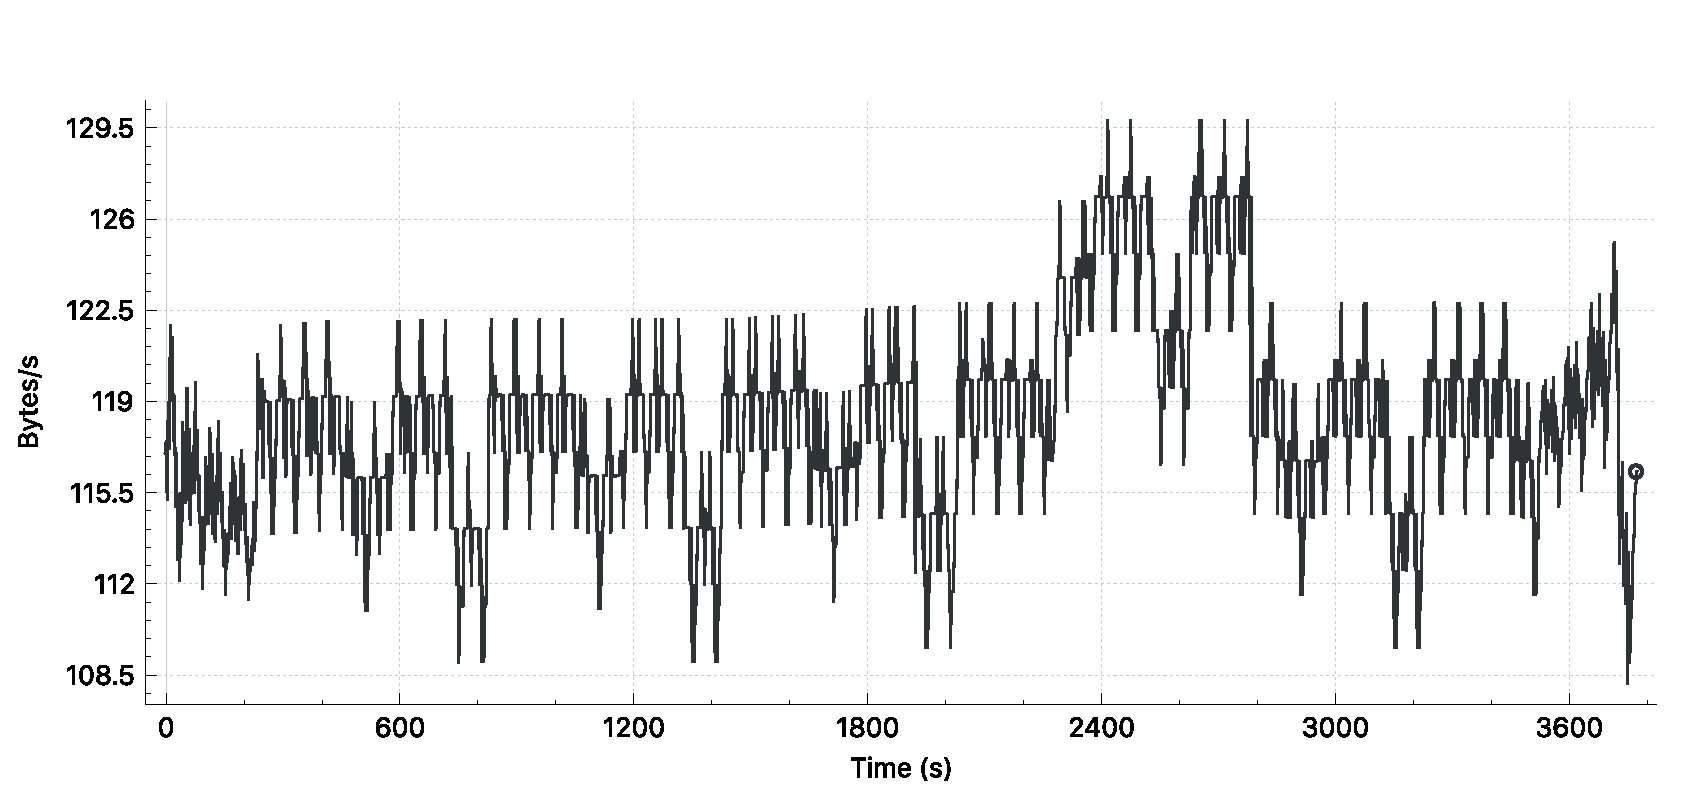
\includegraphics[scale=0.44]{images/test-1h-rsys-solidoff}
	\caption[Vytížení na rsyslogu s aktivovaným škrcením zpráv]{Vytížení na rsyslogu s aktivovaným škrcením zpráv}
\end{figure}


\subsection*{Zhodnocení}
První graf znázorňuje, kolik bitů textu za sekundu daný skript ve skutečnosti generuje.
Zbylé dva grafy už pouze demonstrují, že škrcení funguje správně. Tedy, že tok bitů za sekundu nepřekročí hranici 150 000.

Skript simuluje chování běžných aplikací STB tím, že zprávy které generuje, mají délku odpovídající průměrné délce zpráv generovaných STB.
TODO -- grafy pouze ilustrační, protože realita je jiná. - TODO

\subsection{Vytížení systému}

\section{Zátěžový test v běžných podmínkách}
TODO test využití CPU, old vs new.


\begin{conclusion}

\end{conclusion}

\bibliographystyle{csn690}
\bibliography{mybibliographyfile}

\appendix

\chapter{Seznam použitých zkratek}
\begin{description}
	\item[API] Application Programming Interface
	\item[ASH] Almquist Shell
	\item[CPU] Central Processing Unit
	\item[dmd] Download manager daemon
	\item[GPU] Graphics processing unit
	\item[OS] Operating system
	\item[PC] Personal computer
	\item[RAM] Random Access memory
	\item[RFC] Request for Comments
	\item[SDK] Software Development Kit
	\item[STB] Set-top box
\end{description}

\chapter{Obsah přiloženého CD}

\begin{figure}
	\dirtree{%
		.1 readme.txt\DTcomment{stručný popis obsahu CD}.
		.1 exe\DTcomment{adresář se spustitelnou formou implementace}.
		.1 src.
		.2 impl\DTcomment{zdrojové kódy implementace}.
		.2 thesis\DTcomment{zdrojová forma práce ve formátu \LaTeX{}}.
		.1 text\DTcomment{text práce}.
		.2 thesis.pdf\DTcomment{text práce ve formátu PDF}.
		.2 BP\_Vavricka\_David\_2016.pdf\DTcomment{text práce ve formátu PDF}.
	}
\end{figure}

\end{document}
